%%%%%%%%%%%%%%%%%%%%%%%%%%%%%%%%%%%%%%%%%%%%%%%%%%%%%%%%%%%%%%%%%%%%%%%%%%%%%%%%%%%%%%%%%
% LICENSE NOTICE (CC BY 4.0)
%
% Author/Creator: Alexander Menzel
% Copyright: 2025 MiraTherm
%
% This work is licensed under the Creative Commons Attribution 4.0 International License.
% License Text (URI): https://creativecommons.org/licenses/by/4.0/
%%%%%%%%%%%%%%%%%%%%%%%%%%%%%%%%%%%%%%%%%%%%%%%%%%%%%%%%%%%%%%%%%%%%%%%%%%%%%%%%%%%%%%%%%

\chapter{Concept}
\label{chap:Concept}
In this chapter, the overall concept and approach for the development of the radiator thermostat software is described. Additionally, the required hardware for development and testing is outlined.

\section{Solution approach}
\label{sec:Solution approach}
In this project, a basic software for the device should be implemented including hardware drivers and general program logic. The description of the eQ-3 eqiva Bluetooth from \cite{eQ3AG.05.2018} will be used as a reference for defining the functional scope of the software to be developed.

The software should be designed ready for prospective integration of the control algorithms and Matter-over-Thread standard. (For further details about this standard see \cite{enwiki:matter}.) The device is supposed to be used for smart home applications, specifically for the integration of the thermostat in Home Assistant, smart home applications and/or custom \acp{api}.

\section{Hardware requirements}
\label{sec:Hardware requirements}

To ensure a degree of independence from the \acs{pcb} design and mechanics, the software will be developed using a hardware set that resembles the final thermostat in terms of components and interfaces. This approach enables early software development and testing before the final \acs{pcb} is available.

\subsection{Hardware block diagram}
\label{sec:Hardware block diagram}

A block diagram of the hardware setup for software development and testing is shown in Figure \ref{fig:mt-rt-sw-dev-hw-block-diagram}. Further, a list of required components is provided in section \ref{sec:Required equipment}.

\begin{figure}[htbp]
    \centering
    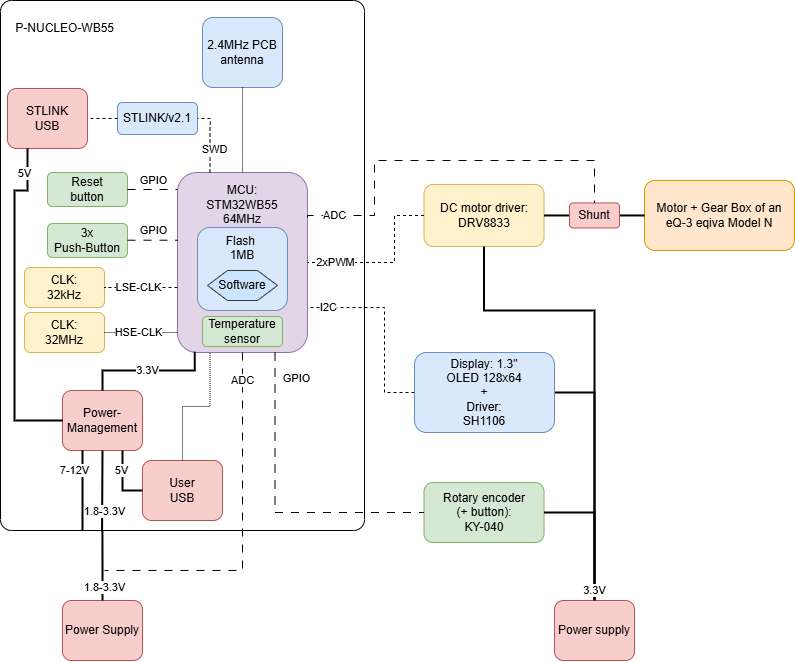
\includegraphics[width=1.0\textwidth]{../../electronics/mt-rt-sw-dev-hw-block-diagram.png}
    \caption{Hardware block diagram of the hardware set for software development and testing}
    \label{fig:mt-rt-sw-dev-hw-block-diagram}
\end{figure}

\subsection{Required equipment}
\label{sec:Required equipment}

For the software development and testing, the following hardware components are required:

\begin{itemize}
    \item \textbf{P-NUCLEO-WB55} - \acs{mcu} development board with Matter standard support
    \item \textbf{eQ-3 eqiva Model N} - Radiator thermostat with a C300 3V motor and gear box for disassembly (available)
    \item \textbf{DRV8833} - Motor driver module
    \item \textbf{Shunt resistor} - For current measurement of the motor
    \item \textbf{1.3" OLED Display incl. SH1106} - Display with an embedded driver
    \item \textbf{KY-040} - Rotary encoder
    \item \textbf{Connecting wires}
    \item \textbf{Breadboard(s)}
\end{itemize}
